\documentclass{article}
\usepackage[utf8]{inputenc}
\usepackage{geometry}
\usepackage{hyperref}
\usepackage{xcolor} 
\usepackage{graphicx}
\geometry{a4paper, margin=1in}

\title{Einrichtungserrors}
\author{}
\date{}

\begin{document}

\maketitle
\noindent\textbf{Unten sind die Errors und Methoden sowie Bemerkungen und mögliche Lösungen, die ich bei der Einrichtung von Jetson Orin Nano 8GB bekommen bzw. umgestzt habe.}
\section{Genutzte Hardware für Image-Flashen}

Folgende Software wurde auf zwei Laptops ausgeführt. Der eine ist ein Hochschul-Laptop. Der andere ist mein persönlicher Laptop. 

\subsection{Hochschul-Laptop}
\begin{itemize}
    \item \textbf{Betriebssystem}: Windows 10
    \item \textbf{Speicher}: 237GB
    \item \textbf{RAM}: 8GB
    \item \textbf{Weiteres}: Core i3, 2 Kerne, 4 logische Prozessoren
\end{itemize}

\subsection{Persönlicher Laptop}
\begin{itemize}
    \item \textbf{Betriebssystem}: Windows 10
    \item \textbf{Speicher}: 222GB SSD + 1TB DDR
    \item \textbf{RAM}: 16GB
    \item \textbf{Weiteres}: Core i5, 4 Kerne, 8 logische Prozessoren
\end{itemize}

\newpage
\section{Errors-Liste und mögliche Lösungen und Empfehlungen}
\begin{enumerate}

    \item \textbf{SD Card Formatter:}\\
    Falls die Anwendung nicht funktioniert, kann dies am Laptop liegen. Versuchen Sie die Anwendung auf einem anderen Laptop zu nutzen. Auf dem Hochschul-Laptop funktioniert sie nicht, auf meinem persönlichen Laptop jedoch schon.
    \par \bigskip
    \item \textbf{Etcher:}
    \begin{itemize}
        \item Falls der Flash-Prozess nicht startet, nutzen Sie einen Laptop mit besserem RAM und CPU. Auf dem Hochschul-Laptop hatte ich dieses Problem, auf meinem persönlichen Laptop nicht.
        \item Falls Etcher zum Blue Screen führt, stellen Sie sicher, dass nur Etcher läuft.
    \end{itemize}
    \par \bigskip

    \item \textbf{Rufus:}
    \begin{itemize}
        \item Falls Etcher nicht funktioniert, nutzen Sie Rufus zum Flashen des Images.
        \item Falls Rufus zum Blue Screen führt, formatieren Sie zuerst die SD-Karte und verwenden Sie dann Rufus.
    \end{itemize}
    \par \bigskip

    \item \textbf{Win32 Disk Manager:}\\
    Falls die SD-Karte nicht erkannt wird, starten Sie den Laptop neu oder versuchen Sie es auf einem anderen Laptop. Auf dem Hochschul-Laptop hatte ich dieses Problem, auf meinem persönlichen Laptop jedoch nicht.
    \par \bigskip

    \item \textbf{Flash-Prozess:}\\
    Wenn das Image erfolgreich geflasht wurde, aber das System nicht bootet und der Bildschirm schwarz bleibt, lesen Sie im \textcolor{blue}{\href{https://forums.developer.nvidia.com/t/jetson-orin-nano-boot-issue-blank-screen-after-nvidia-logo/309412}{Forum}}.
    \par \bigskip

    \item \textbf{DD-Methode:}\\
    Falls der Flash-Prozess weiterhin fehlschlägt, nutzen Sie die DD-Methode unter Ubuntu mit VirtualBox.
    \par \bigskip

    \item \textbf{Speicherplatz-Mängel:}
    Um den Speicher der virtuellen Maschine zu vergrößern, gehen Sie in VirtualBox zu "Virtuelle Medien". Sehen Sie das Bild:
    \par \bigskip

    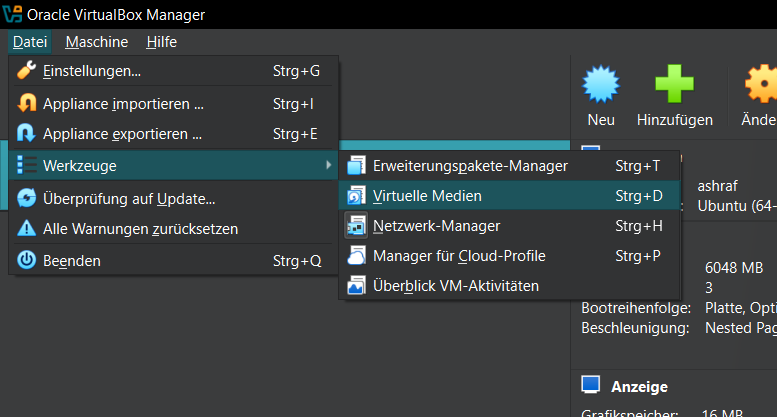
\includegraphics[width=0.8\textwidth]{Errors_Images/VirtuelleMedien.png}

    Nutzen Sie GParted unter Ubuntu, um die Partition zu erweitern. Wählen Sie die Partition, die der SDK Manager verwendet, und klicken Sie auf "resize/move".
    \par \bigskip

    \item \textbf{SDK Manager:}
    \begin{itemize}
        \item Stellen Sie sicher, dass die Hardware im Recovery-Mode ist, indem Sie die Pins \texttt{GROUND} und \texttt{REC} verbinden.
        \item Fügen Sie die USB-3-Schnittstelle in VirtualBox hinzu. Sehen Sie das folgende Bild: 
        \par \bigskip
        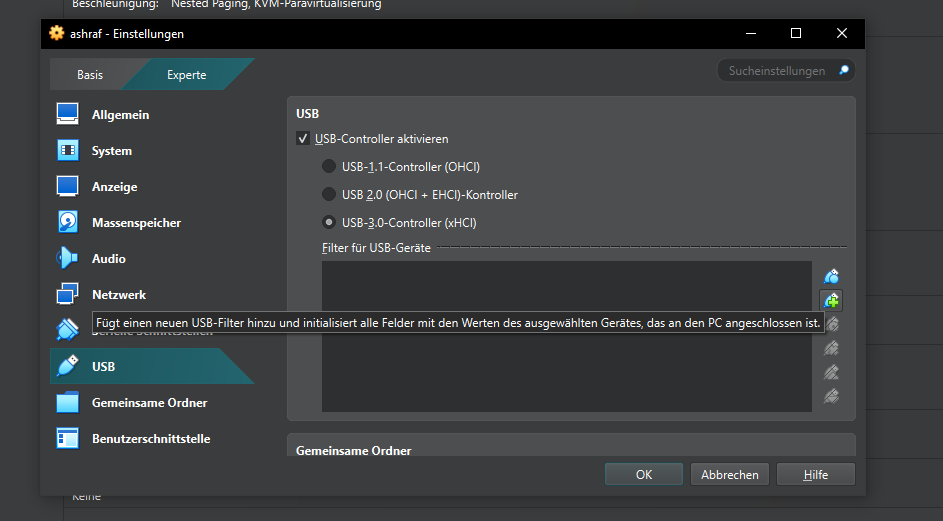
\includegraphics[width=0.8\textwidth]{Errors_Images/Adding_USB.png}
        
    \end{itemize}

    \item \textbf{Zusammenfassung und Lösung:}\\
    Das Hauptproblem lag darin, dass das Image von NVidia zu neu für die Hardware war. Laden Sie JetPack 5 herunter, flashen Sie das Image und booten Sie. Danach können Sie das neue Image verwenden.
    \par \bigskip

\end{enumerate}

\end{document}
